\section{Usability}
This chapter explains how to install and use the tool \Tool.

\subsection{Installation}
This section explains how to install the tool \Tool.
\begin{itemize}[leftmargin=*]
	\item Install a Python Interpreter (version 2.7 or 3).
				You may want to install a distribution (e.g. Python(x,y)) which contains already many useful packages.
	\item The tool \Tool will be delivered in a zipped folder \Code{Toro.zip}. 
				This folder has the following content:
				\begin{itemize}
				\item \textbf{Main script \Code{toro\_main.py}}, 
				\item \textbf{Libraries (pycpa, toro) in the folder \Code{libs}}.
				The libraries under \Code{./libs} are dynamically included. 
				They do not need to be installed unless you want to change their location.
				\item \textbf{Input folder \Code{data}.} Systems to be analyzed can be stored here.
				\end{itemize}
	\item Unzip the zip folder to your preferred destination.	
\end{itemize}


\subsection{Use}
This section gives an overview how to use the tool \Tool.
\begin{itemize}
\item Open a terminal and change to the \Code{/Toro} folder.	
\item The tool \Tool is called via the script \Code{toro\_main.py}.
A path is passed to the script as an argument to specify the location of the system to be analyzed.
It is recommended to store the system to be analyzed in the provided \Code{data} folder.
If several systems are to be analyzed, a subfolder can be created in \Code{data} for each system to be analyzed. 
The folder structure is illustrated in Figure \ref{fig:structure}.
\item An exemplary call of the tool would then look as follows:
\begin{tcolorbox}
\Code{\textbf{user@computer:\textasciitilde/Toro\$} python toro\_main.py ./data}
\end{tcolorbox}
%
\item The tool \Tool then executes, searching for specified systems. 
From the set of found systems, one ore more can interactively be selected for analysis.
Then the same procedure is repeated for each system to be analyzed:
\begin{itemize}
	\item User query to identify the type of system and verify assumptions about the system.
	\item Parsing the csv-files which specify the system (see Section \ref{sec:input-files}.
	\item Calculation of maximum end-to-end latencies and robustness margins.
	\item Generation of diagrams.
	\item Creation of a file containing numerical results.  
	The file is written to the folder in which the analyzed system is specified.
\end{itemize}
\end{itemize}
%
\begin{figure}[t]
		\centering
				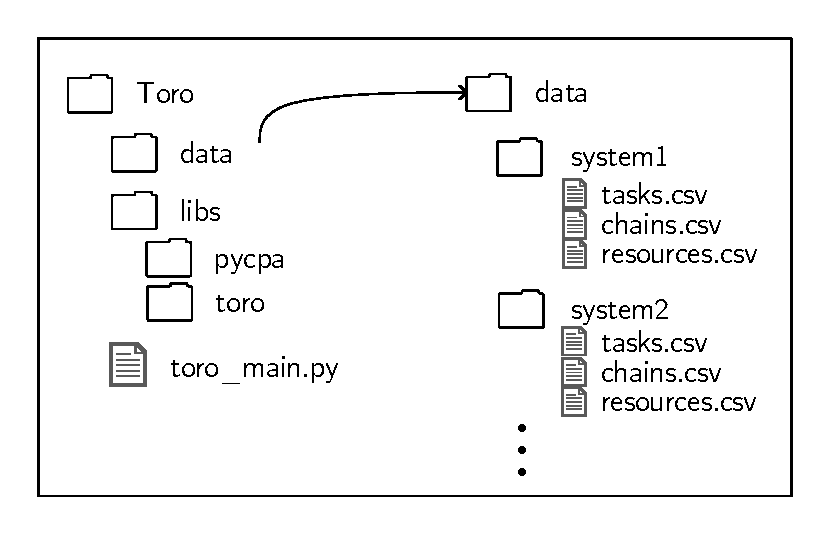
\includegraphics[trim=0.5cm 0.5cm 0.5cm 0.5cm, height=6cm]{fig/structure.pdf}
		\caption{Folder structure}
		\label{fig:structure}
\end{figure}
%


\subsection{Inputs}
\label{sec:input-files}
This section explains how to specify systems that the tool \Tool should analyze.
\bigskip

Firstly, \Tool calls the method \Code{get\_system\_dirs(dir)} and searches the specified folder for systems to be analyzed. 
Each individual system should be encapsulated in a dedicated folder as illustrated in Figure \ref{fig:structure}.
This system folder should contain three semicolon-separated csv-files, namely
\begin{itemize}[itemsep=0pt]
	\item \Code{chains.csv}, 
	\item \Code{resources.csv}, 
	\item \Code{tasks.csv}. 
\end{itemize}
These files can be created in Microsoft Excel, for example, and can then be exported as CSV files.
If \Tool finds more than one system in the specified top-level folder (e.g. \Code{.\\data}), the user can choose from a list which system(s) should be examined. 
An example output would look like this:
\begin{tcolorbox}
\small
{\Code{The following systems have been found:\\
\hspace*{15mm}1: system1\\
\hspace*{15mm}2: system2\\
\hspace*{15mm}2: system3\\
\hspace*{15mm}0: all\\
To select systems enter their ID or a comma-separated list of IDs. For instance, enter 1 to select the first of the listed systems, enter 1,3 to select the first and the third of the listed systems, or enter '0' to select all systems:}}
\end{tcolorbox}

The following sections \ref{sec:input-files-resources}-\ref{sec:input-files-chains} explain the structure of the CSV files. 
Then sections \ref{sec:input-files-bet1}-\ref{sec:input-files-let} demonstrate the three possible types of use cases and which information needs to be filled in.


\subsubsection{Input File 'resources.csv'}
\label{sec:input-files-resources}
The \Code{resources.csv} file describes the execution platform of the system by listing the different resources (CPUs, CAN bus etc.) and the scheduling policy that is applied on each resource. 
%Currently static priority preemptive and static priority non-preemptive scheduling is supported.
The \Code{resources.csv} file should have the following column headers:
\begin{description}
		\item [name] Type: String \hfill \\ 
		Each computing core and each data bus, on which at least one chain task is executed, is represented by a so-called \emph{resource}.   This field specifies the name of the resource.		
		\item [scheduler] Type: String \hfill \\ 
		e.g., \Code{SPPScheduler} or \Code{SPNPScheduler}
\end{description}
\bigskip


\subsubsection{Input File 'tasks.csv'}
\label{sec:input-files-tasks}
The \Code{tasks.csv} file specifies tasks that are executed on the platform, it should have the following column headers:
\begin{description}
		\item [task\_name] Type: String \hfill \\ 
		Unique task ID
		\item [period] Type: Integer \hfill \\ 
		Activation period		
		\item [offset] Type: Integer \hfill \\ 
		Release offset
		\item [priority] Type: Integer \hfill \\ 
		Note that 0 is the highest priority.
		\item [wcet] Type: Integer \hfill \\ 
		Worst Case Execution Time		
		\item [resource] Type: String \hfill \\ 
		Resource that services the task. 
		The name should match a resource from file \Code{pycpa\_resources.csv}.
		\item [bcrt] Type: Integer \hfill \\ 
		Best Case Response Time		
		\item [wcrt] Type: Integer \hfill \\ 
		Worst Case Response Time
		\item [let] Typ: Integer \hfill \\ 
		Logical Execution Time 
\end{description}
\bigskip


\subsubsection{Input File 'chains.csv'}
\label{sec:input-files-chains}
The \Code{chains.csv} file specifies which tasks are part of each cause-effect chain; it should have the following column headers:
\begin{description}
		\item [chain\_name] Type: String \hfill \\ 
		Unique cause-effect chain ID
		\item [e2e\_deadline] Type: Integer \hfill \\ 
		End-to-end deadline 		
		\item [members] Type: String \hfill \\ 
		The member tasks must be listed in correct order and the task names must match those in the task definitions. The list of member tasks comprises as many cells in a row as needed.
\end{description}



\newpage
\subsubsection{Use Case 1:Cause-effect chains with BET tasks, WCRT for each chain task known}
\label{sec:input-files-bet1}

\begin{tcolorbox}
\begin{itemize}[leftmargin=*, itemsep=0pt]
	\item applicable to many systems
	\item the name, period, offset, WCRT of every task in a cause-effect chain must be known
\end{itemize}
\end{tcolorbox}
\bigskip

For \emph{Use Case 1} given that
\begin{itemize}[leftmargin=*, itemsep=0pt]
	\item all clocks in the system are synchronized,
	\item all tasks in the cause-effect chains are BET tasks,
	\item task deadlines are implicit,
\end{itemize}
(which is checked in an interactive user query), 
it is sufficient to specify the following details of the entire systems.
An example system of type \emph{'Use Case 1'} is depicted in Figure \ref{fig:use-case-1}.

For the example system, the file \Code{resources.csv} would contain:
\begin{center}
	\begin{tabular}{|l|l|} \hline
		\textbf{name} & \textbf{scheduler} \\ \hline
		unknown & unknown \\ \hline
	\end{tabular}
\end{center}
With regard to the tasks that are part of the cause-effect chains to be analyzed, we have in \Code{tasks.csv} 
\begin{center}
	\begin{tabular}{|l|l|l|l|l|l|l|l|l|} \hline
		  \textbf{task\_name}  
		& \textbf{period} 
		& \textbf{offset} 
		& \textbf{priority}
		& \textbf{wcet}
		& \textbf{resource} 
		& \textbf{bcrt}		
		& \textbf{wcrt}
		& \textbf{let} \\ \hline
	\end{tabular}
\end{center}
Note that a number of fields in \Code{resources.csv} and \Code{tasks.csv} can be left empty or declared as 'unknown' because the WCRTs are already available and do not need to be computed from these parameters.
\bigskip

The cause-effect chains in \Code{chains.csv} are specified by
\begin{center}
	\begin{tabular}{|l|l|l|l|l|} \hline
		\textbf{chain\_name} 
		& \textbf{e2e\_deadline}
		& \multicolumn{3}{|l|}{\textbf{members}} \\ \hline
	\end{tabular}
\end{center}
%
\begin{figure}[h!]
	\centering
		\includegraphics[width=0.7\textwidth,page=2]{fig/example_input.pdf}
	\caption{Use case 1; relevant parts of the system for the analysis are marked in color.}
	\label{fig:use-case-1}
\end{figure}



\newpage
\subsubsection{Use Case 2: Cause-effect chains with BET tasks,\\ WCRT of each chain task computable}
\label{sec:input-files-bet2}

\begin{tcolorbox}
\begin{itemize}[leftmargin=*, itemsep=0pt]
	\item only applicable to systems with \ac{spp} und \ac{spnp} scheduling
	\item not only tasks that are part of cause-effect chains must be specified but also the entire background load with all parameters
\end{itemize}
\end{tcolorbox}

For \emph{Use Case 2} given that
\begin{itemize}[leftmargin=*, itemsep=0pt]
	\item all clocks in the system are synchronized,
	\item ALL tasks are BET tasks (not only those in the listed cause-effect chains),
	\item task deadlines are implicit,	
	\item ALL tasks in the system must be known with their parameters,
	\item ALL resources must be known with their scheduling algorithms (SPP or SPNP) and the task-to-resource mapping,
\end{itemize}
(which is checked in an interactive user query), 
it is sufficient to specify the following details of the entire systems.
An example system of type \emph{'Use Case 2'} is depicted in Figure \ref{fig:use-case-2}.
For the example system, the file \Code{resources.csv} would contain:

\begin{center}
\small
	\begin{tabular}{|l|l|} \hline
		\textbf{Name} & \textbf{Scheduler} \\ \hline	
	\end{tabular}
\end{center}

With regard to the tasks that are part of the cause-effect chains to be analyzed, we have not only the chain tasks but also the tasks of the background load with all parameters required to compute the WCRTs.
\begin{center}
	\begin{tabular}{|l|l|l|l|l|l|l|l|l|} \hline
		  \textbf{task\_name}  
		& \textbf{period} 
		& \textbf{offset} 
		& \textbf{priority}
		& \textbf{wcet}
		& \textbf{resource} 
		& \textbf{bcrt}		
		& \textbf{wcrt}
		& \textbf{let} \\ \hline
	\end{tabular}
\end{center}

The cause-effect chains are specified again by
\begin{center}
	\begin{tabular}{|l|l|l|l|l|} \hline
		\textbf{chain\_name} 
		& \textbf{e2e\_deadline}
		& \multicolumn{3}{|l|}{\textbf{members}} \\ \hline
	\end{tabular}
\end{center}
%
\begin{figure}[h!]
	\centering
		\includegraphics[width=0.7\textwidth,page=3, trim = 0.5cm 0.5cm 0.5cm 0.5cm]{fig/example_input.pdf}
	\caption{Use case 2; relevant parts of the system for the analysis are marked in color}
	\label{fig:use-case-2}
\end{figure}


\newpage
\subsubsection{Use Case 3: Cause-effect chains with LET tasks, LET for each chain task known}
\label{sec:input-files-let}
%

\begin{tcolorbox}
\begin{itemize}[leftmargin=*, itemsep=0pt]
	\item applicable to LET systems
\end{itemize}
\end{tcolorbox}
\bigskip

For \emph{Use Case 3} given that
\begin{itemize}[leftmargin=*, itemsep=0pt]
	\item all clocks in the system are synchronized,
	\item all tasks in the cause-effect chains are LET tasks,
	\item all LET tasks have implicit deadlines,	
\end{itemize}
(which is checked in an interactive user query), 
it is sufficient to specify the following details of the entire systems.
An example system of type \emph{'Use Case 3'} is depicted in Figure \ref{fig:use-case-3}.

For the example system, the file \Code{resources.csv} would contain:
\begin{center}
	\begin{tabular}{|l|l|} \hline
		\textbf{name} & \textbf{scheduler} \\ \hline
		unknown & unknown \\ \hline
	\end{tabular}
\end{center}
With regard to the tasks that are part of the cause-effect chains to be analyzed, we have in \Code{tasks.csv} 
\begin{center}
	\begin{tabular}{|l|l|l|l|l|l|l|l|l|} \hline
		  \textbf{task\_name}  
		& \textbf{period} 
		& \textbf{offset} 
		& \textbf{priority}
		& \textbf{wcet}
		& \textbf{resource} 
		& \textbf{bcrt}		
		& \textbf{wcrt}
		& \textbf{let} \\ \hline
	\end{tabular}
\end{center}

The cause-effect chains are specified by
\begin{center}
	\begin{tabular}{|l|l|l|l|l|} \hline
		\textbf{chain\_name} 
		& \textbf{e2e\_deadline}
		& \multicolumn{3}{|l|}{\textbf{members}} \\ \hline	
	\end{tabular}
\end{center}
%
\begin{figure}[h!]
	\centering
		\includegraphics[width=0.7\textwidth,page=2]{fig/example_input.pdf}
	\caption{Use case 3; relevant parts of the system for the analysis are marked in color.}
	\label{fig:use-case-3}
\end{figure}


\newpage
\subsection{Outputs}
\label{sec:outputs}
Outputs are written into the folder of the specified system.

\subsubsection{Log File}
The numberical results are written to the text file 
\Code{RESULTS_LOG.txt}.

\subsubsection{Interval Diagram}
%
\begin{figure}
		\centering
		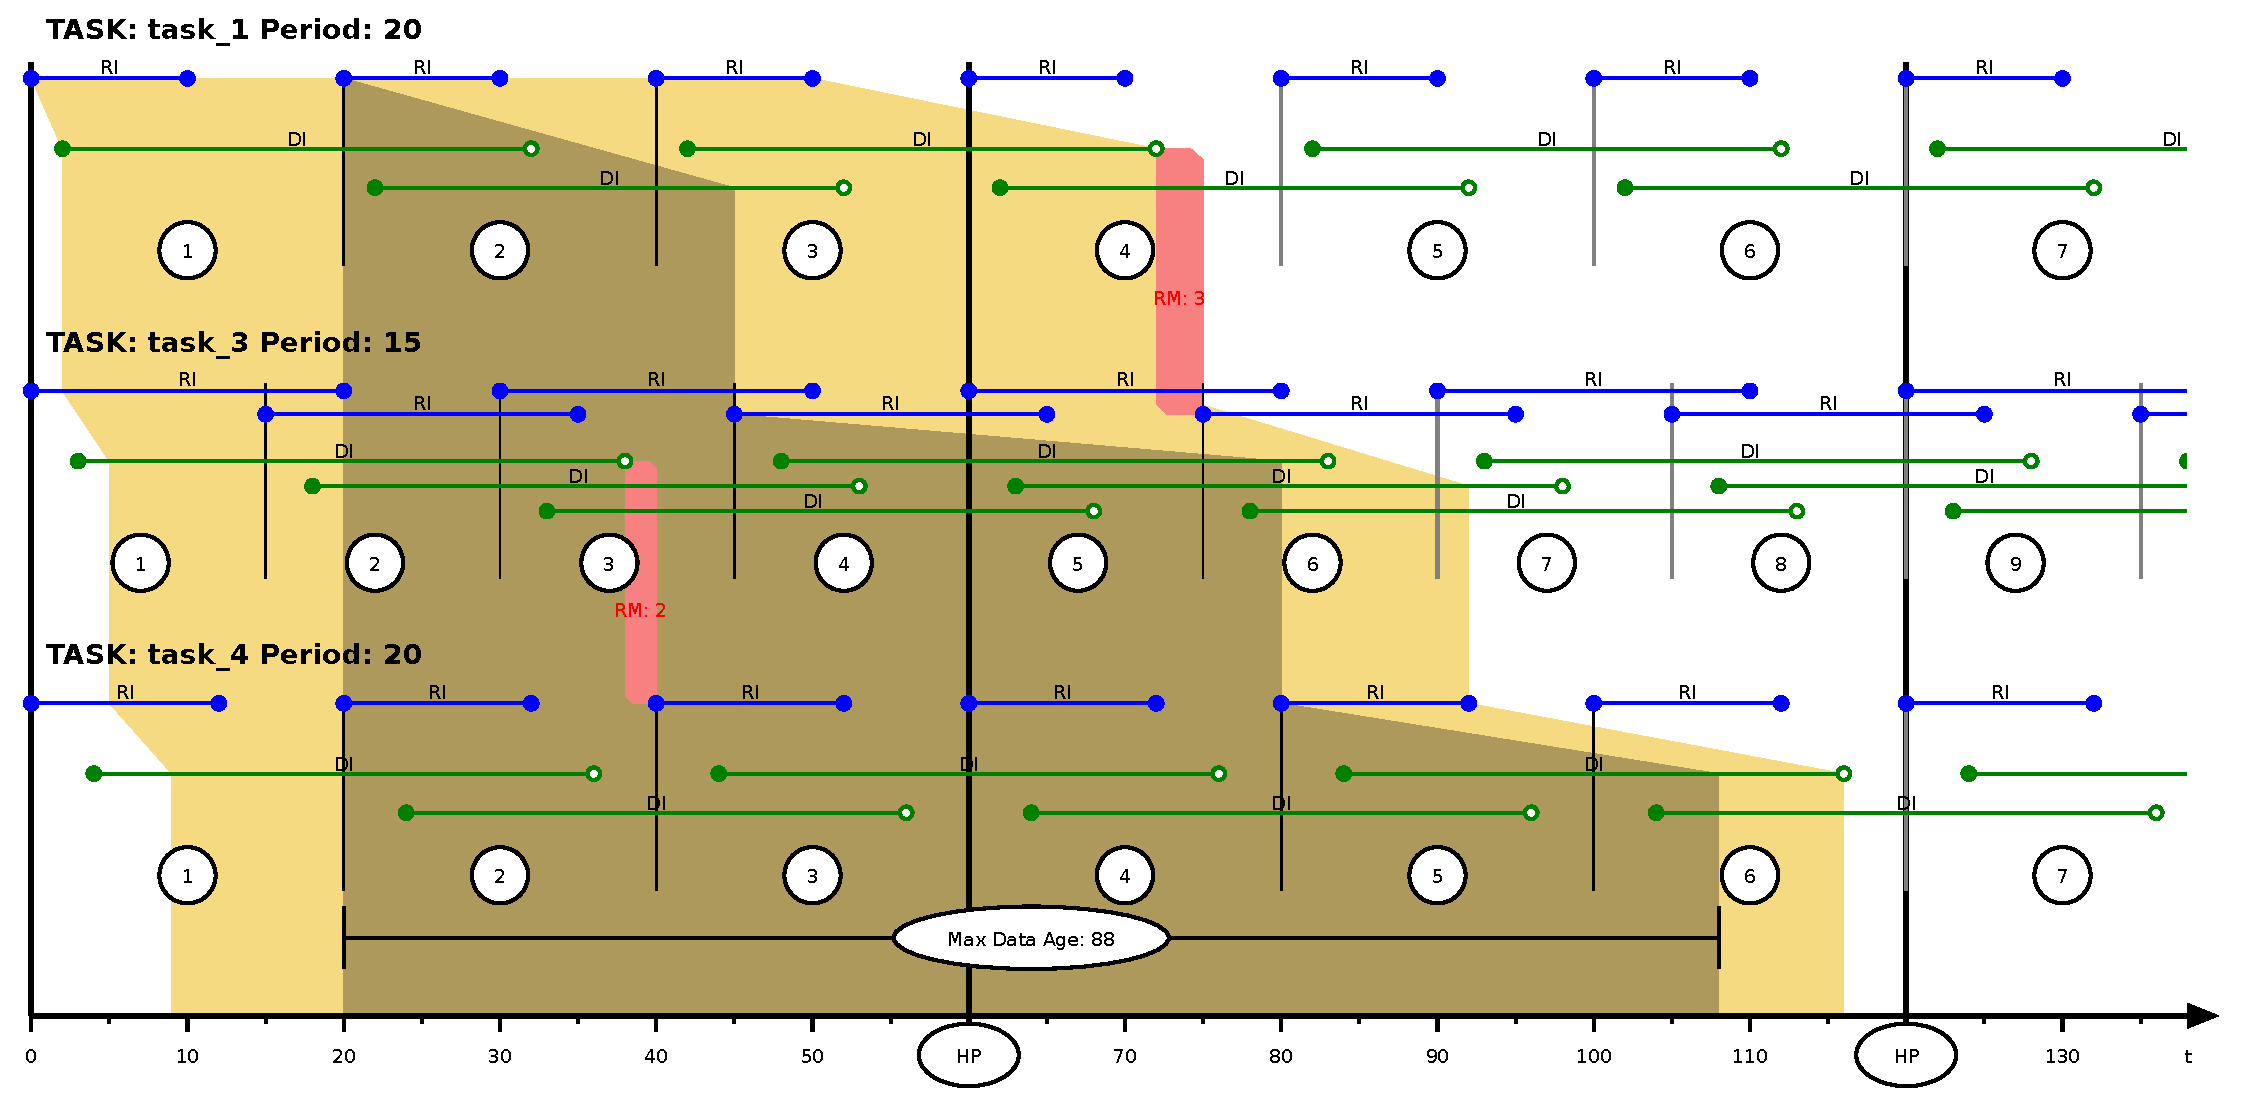
\includegraphics[width=415pt]{fig/intervalls.pdf}
		\caption{Interval diagram.}
		\label{fig:interval_diagram}
\end{figure}
%
In the interval diagram, the individual jobs are represented as numbered circles. 
The blue-marked read intervals represent the earliest possible to latest possible time, when a job can read data. 
The green-marked data intervals bound the period of time in which the output data of a job is available to other jobs.
The short vertical lines stand for the period of a task.
The long vertical lines show the hyper period (HP).
\smallskip

The yellow area covers all instances of the cause-effect chain which are relevant for the computation of the maximum end-to-end latency and the robustness margins. \\
The dark area highlights one instance of a cause-effect chains which actually has the maximum end-to-end latency. \\
The red areas illustrate some selected robustness margins, which are valid for the isolated cause-effect chain (not for the set of specified cause-effect chains in \Code{chains.csv}.


\newpage
\subsubsection{Reachability Graph}
%
\begin{figure}[H]
		\centering
		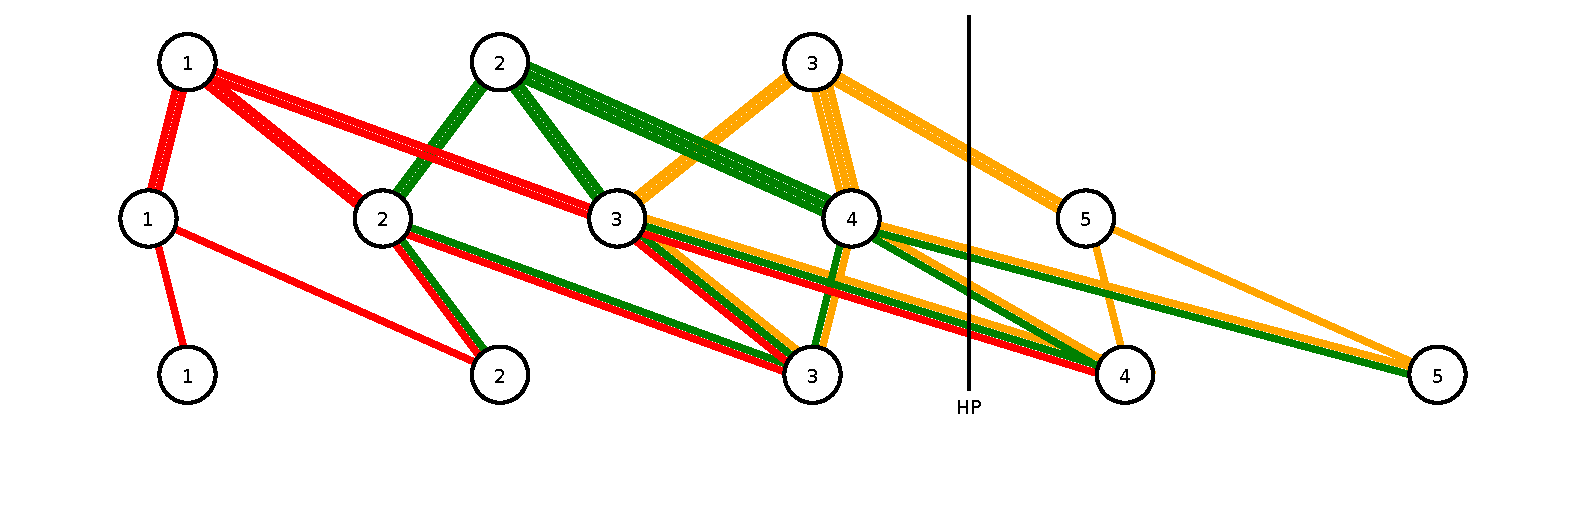
\includegraphics[width=400pt]{fig/tree.pdf}
		\caption{Reachability graph}
		\label{fig:reachability}
\end{figure}
%
The reachability graph results from the overlap of read intervals and data intervals of jobs (data flow analysis). 
In the reachability graph, all possible paths of starting in from the first hyperperiod are represented.
These paths are required for the computation of the maximum end-to-end latency and the robustness margins. 
The colored marking of the individual paths makes it easy to recognize where a path begins and ends. The numbers stand for the respective job number. 
    

\newpage
\subsubsection{Overview Graph}
The overview graph represents the specified cause-effect chains as a tasks with data flow dependencies.
Moreover, it lists the computed maximum end-to-end latencies for each cause-effect chain.
Finally, it indicates the robustness margins for the isolated chains and in the presence of all chains.
%
\begin{figure}[H]
  \centering
  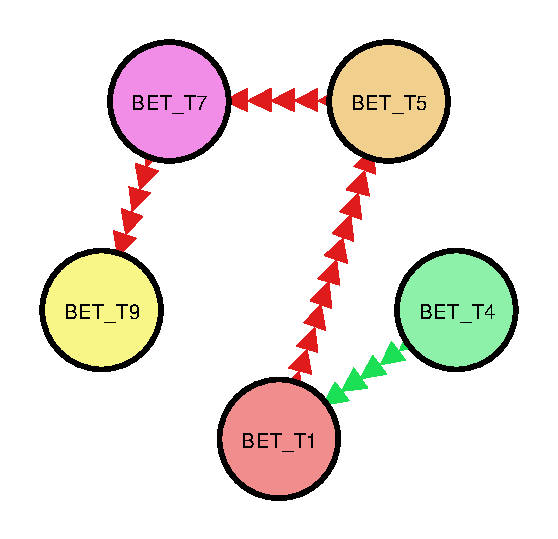
\includegraphics[width=400pt]{fig/results.pdf}
  \caption{Summarizing diagram.}
  \label{fig:summ_diagram}
\end{figure}



\newpage
\section{Internals}

The tool \Tool relies on the Python packages
\begin{itemize}[itemsep=0pt]
	\item \Code{toro}
	\item \Code{pycpa}
\end{itemize}
and the main script
\begin{itemize}[itemsep=0pt]
	\item \Code{toro\_main.py}
\end{itemize}
Details about the \Code{pycpa} package can be found in the online documentation at \url{https://pycpa.readthedocs.io}.
The other two components are discussed in more detail in the following sections \ref{sec:script} and \ref{sec:toro_lib}.
    
\subsection{User Script}
\label{sec:script}
The main script \Code{toro\_main.py} consists of two methods (cf. Figure \ref{fig:toro_internals}):

\paragraph{get\_system\_dirs(dir)}
The script \Code{toro\_main.py} starts with the main method and passes the call parameter (folder path) to the \Code{get\_system\_dirs(dir)} method. \\
The method \Code{get\_system\_dirs(dir)} searches for existing systems under the specified path. 
If more than one system is found, the user can choose from a list which systems should to be analyzed. 

\paragraph{perform\_analysis(dir)}
The method \Code{perform\_analysis(dir)} 
\begin{itemize}[itemsep=0pt]
	\item starts a user query to identify the type of system and verify assumptions about the system,
	\item parses the csv-files which specify the system,
	\item calculates the maximum end-to-end latencies and robustness margins,
	\item generates of diagrams,
	\item logs the numerical results (\Code{RESULTS\_LOG.txt}), 
\end{itemize}
for each of the selected systems.
 %
\begin{figure}[H]
		\centering
		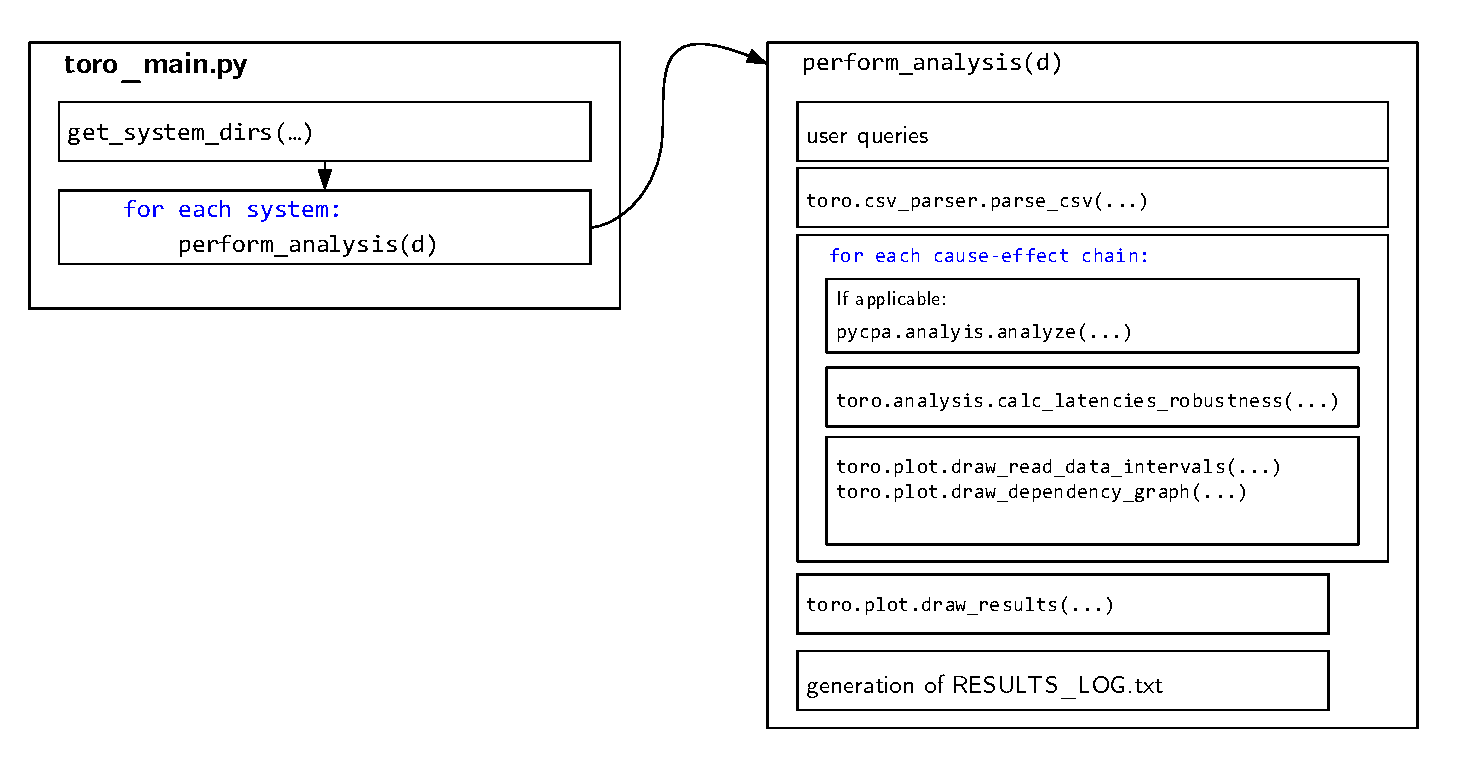
\includegraphics[width=\textwidth]{fig/toro_architecture.pdf}
		\caption{Internals of the main script \Code{toro\_main.py}}
		\label{fig:toro_internals}
\end{figure}

 
\subsection{Toro Package}
\label{sec:toro_lib}
    
This section describes the modules in the package \Code{toro}.

\paragraph{toro.model}
This module defines the data structures required within the software. 
It is an extension of the module of the same name from the \Code{pycpa} package.

\paragraph{toro.analysis}
This module contains the \Code{calc\_latencies\_robustness} class.
When an object of this class is initialized and a chain is passed as an argument, then the maximum latency and the robustness margins for each task are computed.

\paragraph{toro.csv\_parser}
This module reads the CSV-files from the specified folder and transfers them into the software's internal data structure. 
If files are not available or data is not properly defined, an error message is issued. 
The parser is called via the \Code{prase\_csv} class, which requires the folder path of the system to be analyzed as argument.

\paragraph{toro.plot}
The module plots creates graphical representations of the analysis results; the three different types of graphs have been discussed in the section \ref{sec:outputs}.
The module consists of several classes, each is designed for one of the graphical output formats. 

\begin{description}
\item[\Code{image}] 
The \Code{image} class provides the basic functions to draw circles, lines, text and other elements in an SVG image.  
%
\item[\Code{draw\_read\_data\_intervals}] 
This class draws the read and data intervals of jobs in a representative time window on the basis of the analysis results. 
In addition, the computed properties -- maxmimum end-to-end latency and the robustness margins for the isolated chain -- can be drawn using the options "all", "none", "first" and "last". 
A further option is to include the "Dependency Polygon":
\begin{itemize}
		\item max\_data\_age = all | first | last | none
		\item robustness\_margin = all | first | last | none
		\item dependency\_polygon = True | False.
\end{itemize}    
												
\item[\Code{draw\_dependency\_graph}] 
The reachability graph illustrates possible instances of a cause-effect chain. As the call parameter are the analysis results required.
%
\item[\Code{draw\_results}] 
The relevant results of all tasks and cause-effect chains of a system are displayed in an overview graph. 
Chains and tasks are used as call parameters. 
%
\end{description}